\documentclass[paper=a4]{article}
\usepackage{graphicx}
\usepackage[margin=3cm]{geometry}

\begin{document}
    \section{Implementation of Synchronous and Asynchronous 3-bit counters}
    Using the schematic in Figures \ref{fig:e7schemAsync} and \ref{fig:e7schemSync} and  the circuits were implemented on a Printed Circuit Board.

    \begin{figure}[h!]
        \begin{center}
            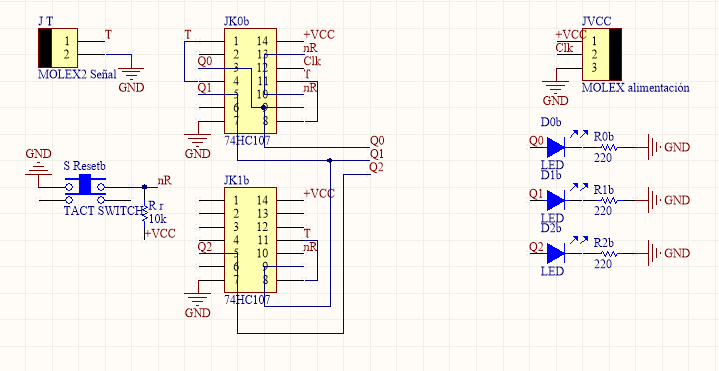
\includegraphics[width=0.6\linewidth]{images/aaschem7async.png}
            \caption{Shcematics for the Asynchronous counter}
            \label{fig:e7schemAsync}
            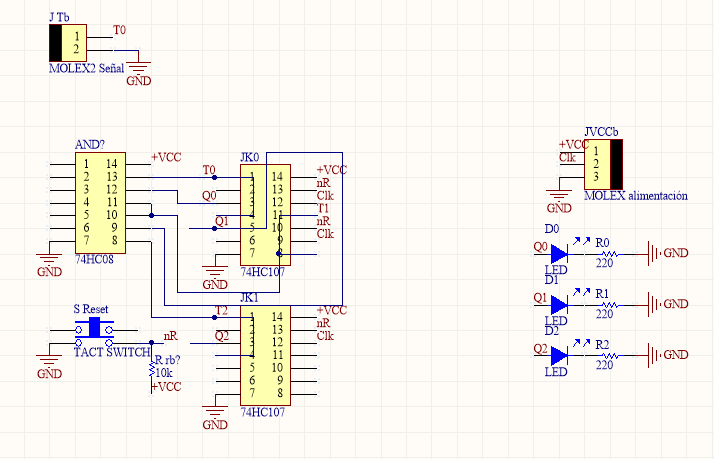
\includegraphics[width=0.6\linewidth]{images/aaschem7sync.png}
            \caption{Schematics for the Synchronous counter}
            \label{fig:e7schemSync}
        \end{center}
    \end{figure}

    First, the behaviour of both devices was verified. Line 1 represents the Clk signal while lines 2, 3 and
    4 represent a binary bit in the counter.
    \begin{figure}[ht]
        \begin{center}
            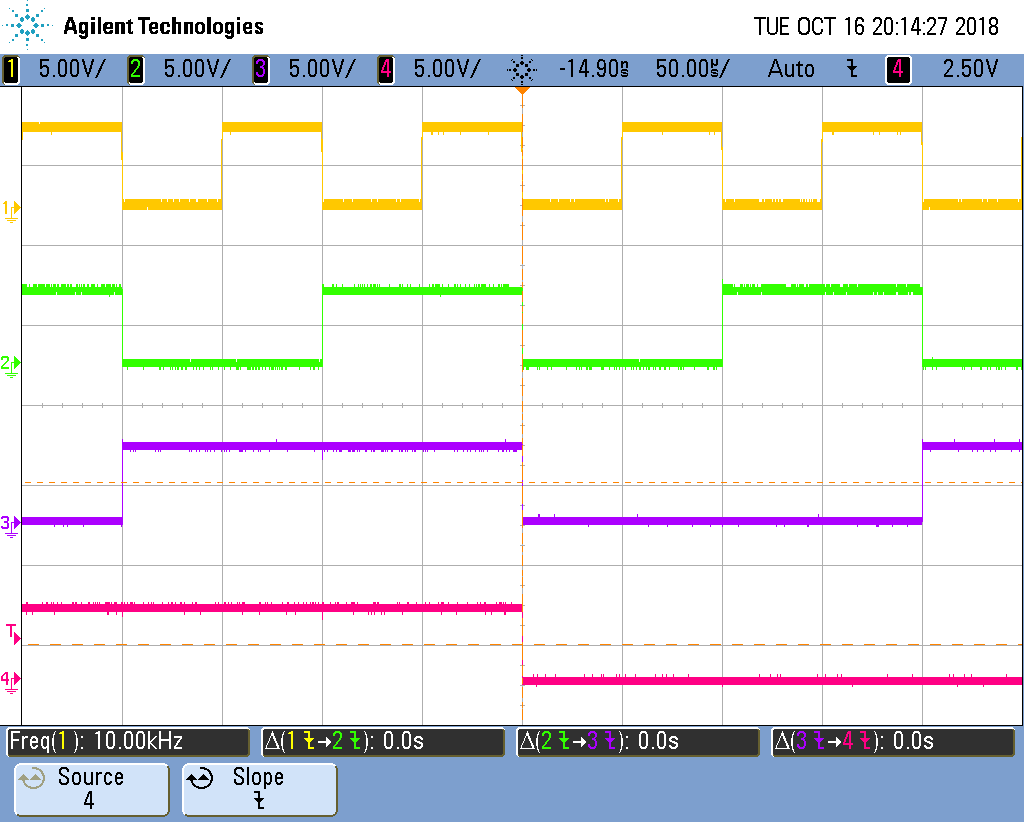
\includegraphics[width=0.6\linewidth]{images/e3_e7_async0.png}
            \caption{Asynchronous counter test on 10 kHz}
            \label{fig:e7asynctest1}
        \end{center}
    \end{figure}

    \begin{figure}[ht]
        \begin{center}
            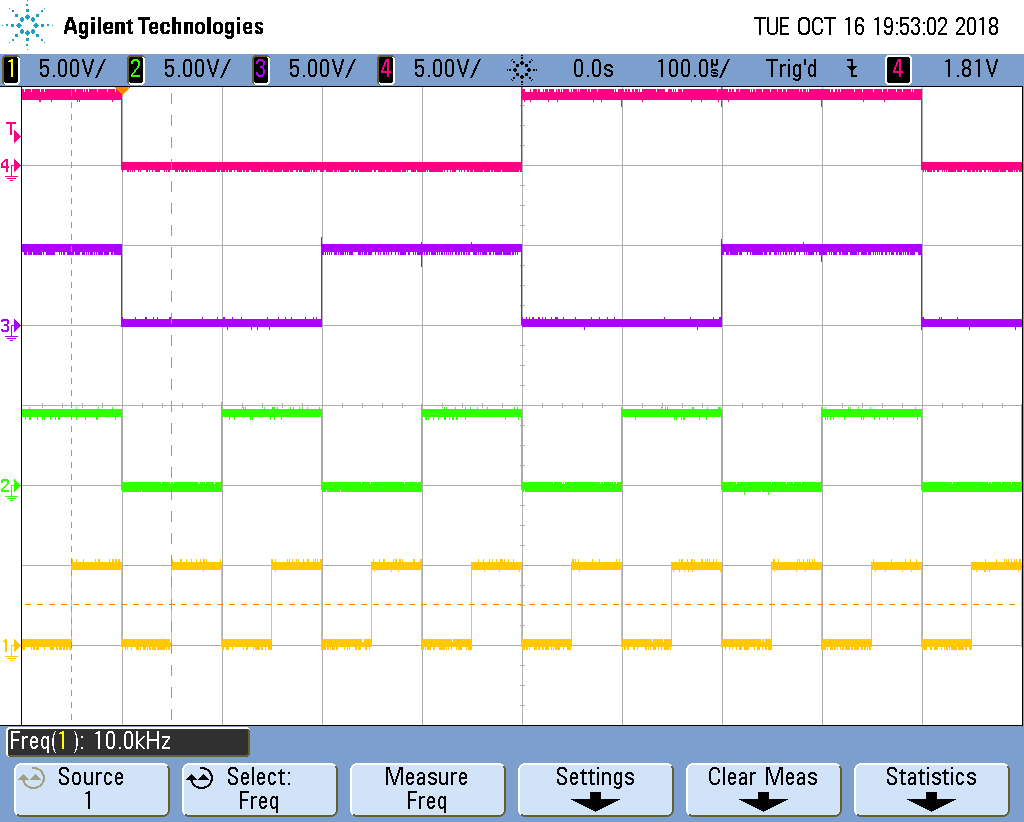
\includegraphics[width=0.6\linewidth]{images/e3_e7_sync4.png}
            \caption{Sinchronous counter test on 10 kHz}
            \label{fig:e7synctest1}
        \end{center}
    \end{figure}

    It can be observed from Figures \ref{fig:e7asynctest1} and \ref{fig:e7synctest1} that at this relatively low frequency, there is no visible difference on
    the behaviour of both counters. However, upon increasing the frequency and measuring the delays
    between each negative edge slope, the differences in operation can be observed.

    \begin{figure}[ht]
        \begin{center}
            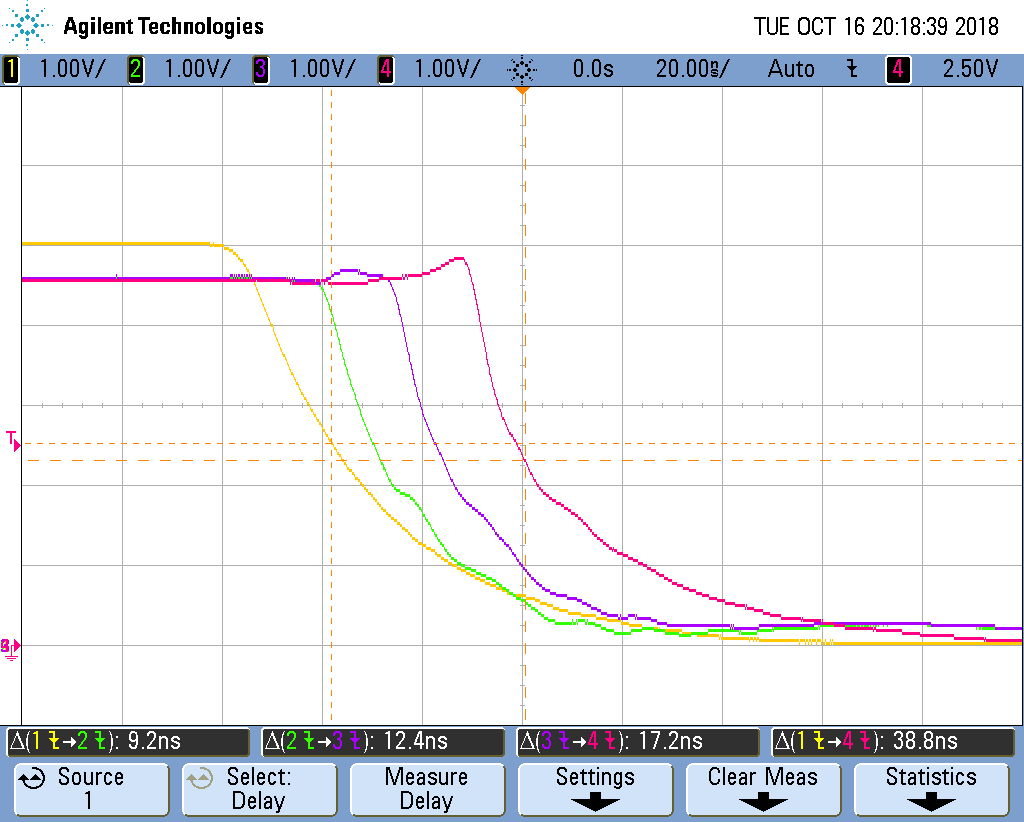
\includegraphics[width=0.6\linewidth]{images/e3_e7_async1mhz.png}
            \caption{Asynchronous counter test on 1 MHz}
            \label{fig:e7asynctest2}
        \end{center}
    \end{figure}

    \begin{figure}[ht]
        \begin{center}
            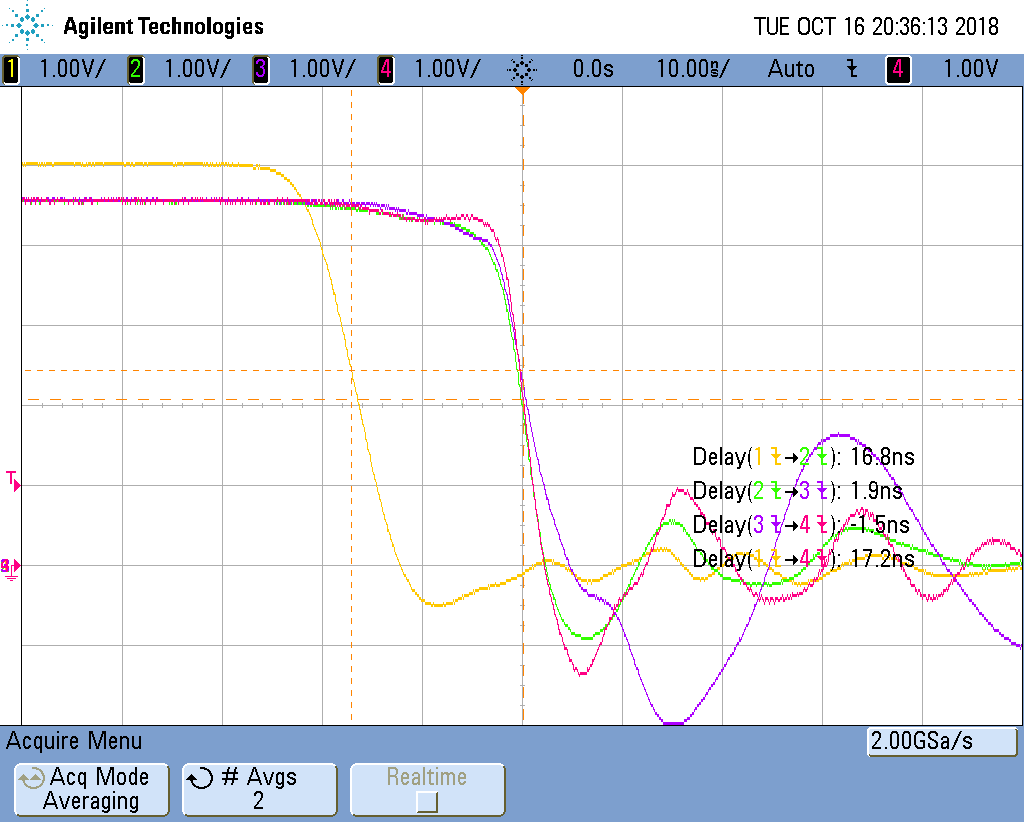
\includegraphics[width=0.6\linewidth]{images/e3_e7_sync_1mhz.png}
            \caption{Synchronous counter test on 1MHz}
            \label{fig:e7synctest2}
        \end{center}
    \end{figure}

    On Figures \ref{fig:e7asynctest2} and \ref{fig:e7synctest2} the difference in behaviour can clearly be seen:
    while on the Asynchronous counter the delay between each subsequent signal is within similar values, in the 
    Synchronous counter there is only significant delay between the clock signal(1) and all the other signals, while
    between signals 2, 3, and 4, is an order of magnitude lower.
    
    When using the maximum available frequency on both counters, one can see the limitations of the Asynchronous 
    configuration: at this frequency, the clock signal and the 3rd bit signal start to overlap (confirmed by the 
    negative measurement of the delay between them in Figure \ref{fig:e7asynctest3}), while the Synchronous configuration's waveforms remain without
    overlap and delays on the positive side of the scale (Figure \ref{fig:e7synctest3}).

    \begin{figure}[ht]
        \begin{center}
            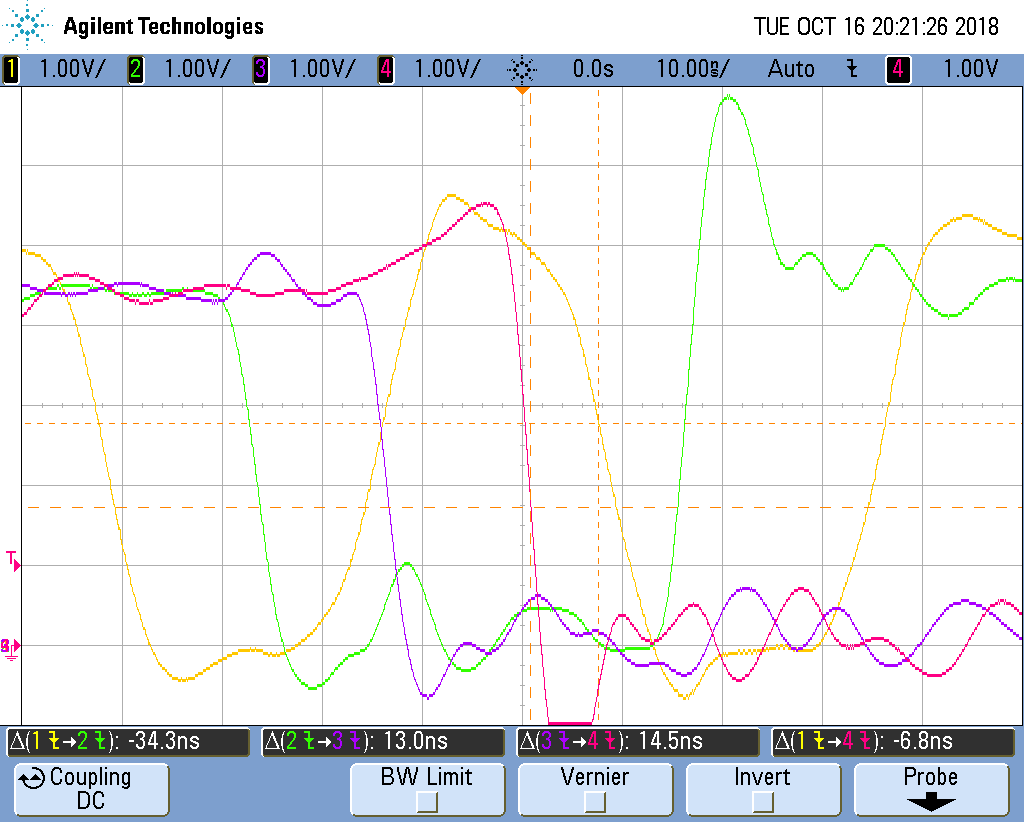
\includegraphics[width=\linewidth]{images/e3_e7_async20mhz.png}
            \caption{Asynchronous counter test on 20 MHz}
            \label{fig:e7asynctest3}
        \end{center}
    \end{figure}

    \begin{figure}[ht]
        \begin{center}
            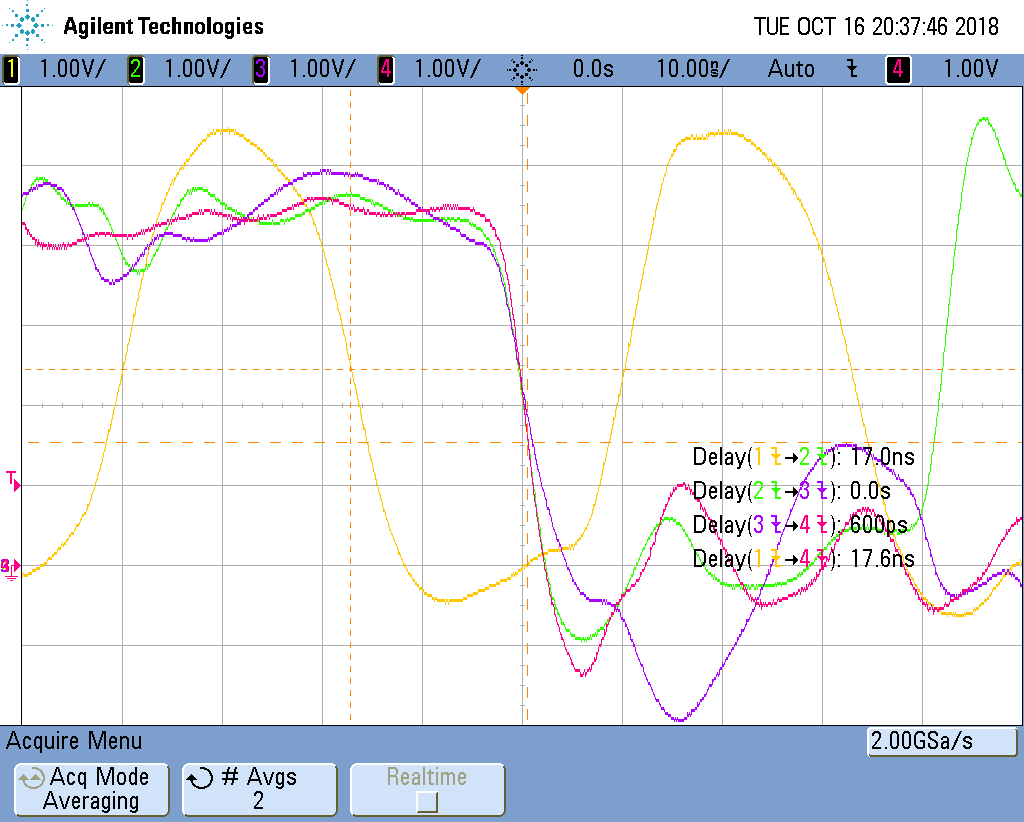
\includegraphics[width=\linewidth]{images/e3_e7_sync_20mhz.png}
            \caption{Synchronous counter test on 20 MHz}
            \label{fig:e7synctest3}
        \end{center}
    \end{figure}

    In conclusion, despite the Asynchronous counter's economical advantage due to the use of fewer components, it
    runs into the limitation that it will stop working properly at high frequencies, while the Synchronous counter,
    despite requiring more components, it continues working properly at much higher frequencies.

\end{document}